\chapter{Materiais e Métodos}\label{cap:metodologia}

Este capítulo apresenta a metodologia e os recursos utilizados no desenvolvimento deste trabalho. A \autoref{sec:espec_maq} descreve as configurações de \textit{hardware} das máquinas empregadas na execução dos experimentos. Em seguida, a \autoref{sec:benchmark} detalha as aplicações selecionadas para os testes, bem como as técnicas de otimização adotadas e o posicionamento das regiões paralelas. A \autoref{sec:desempenho} aborda os métodos utilizados para a coleta e análise dos dados de desempenho. Por fim, a \autoref{sec:resumo_exp} apresenta uma síntese de todos os experimentos realizados, organizada em formato tabular.

\section{Especificações das Máquinas Usadas}\label{sec:espec_maq}

Todos os experimentos deste trabalho foram realizados em um computador equipado com um processador Intel Core i7-4690, com frequência de 3.6 GHz, quatro núcleos físicos e suporte a oito \textit{threads}. A hierarquia de memória \textit{cache} apresenta 32 KB, 256 KB e 8 MB nos níveis L1, L2 e L3, respectivamente. O sistema possui 32 GB de memória RAM DDR3, distribuídos em quatro módulos de 8 GB configurados em \textit{dual-channel}, cada um operando a 1600 MT/s. O sistema operacional utilizado foi o Ubuntu 22.04 LTS. A \autoref{fig:compArchitecture} apresenta a hierarquia de memória e a disposição dos núcleos do processador utilizados nos testes.

\begin{figure}[htb]
	\caption{Especificação do computador utilizado em testes}
	\label{fig:compArchitecture}
	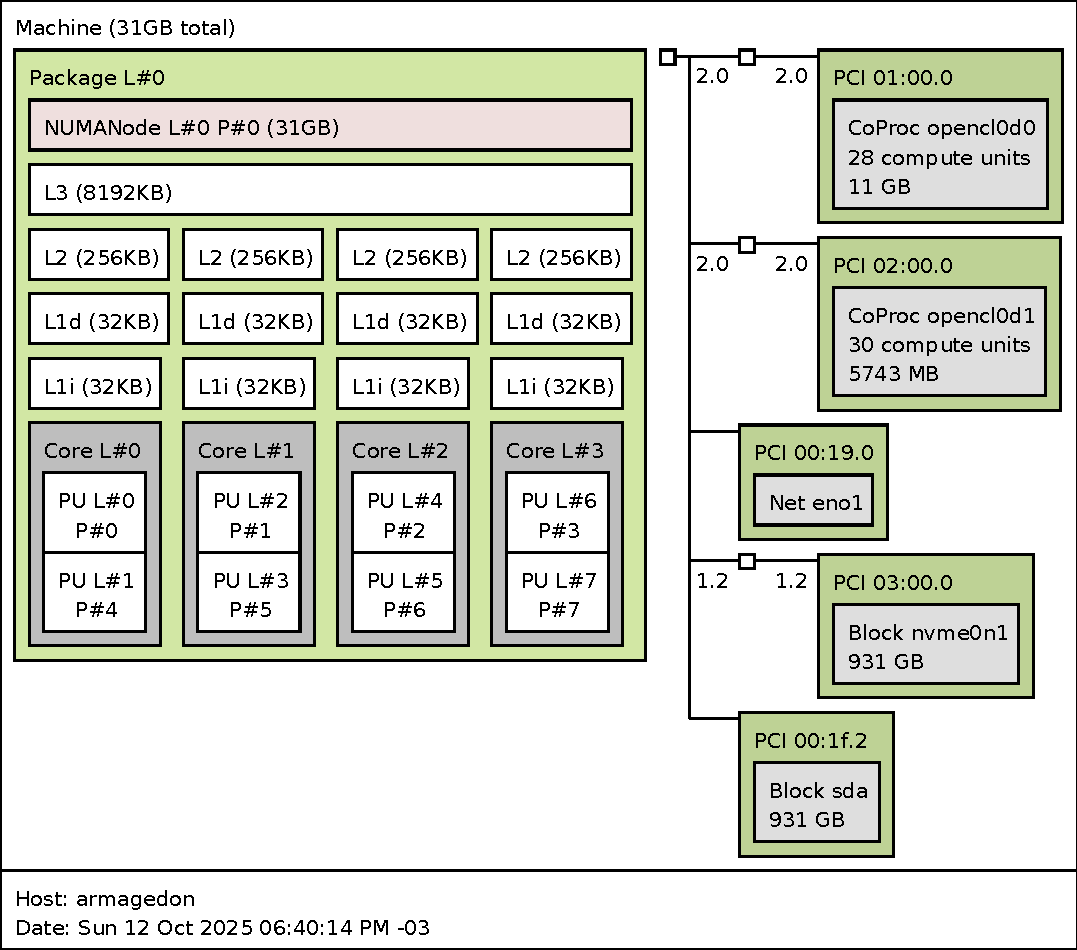
\includegraphics[scale=0.7]{figuras/architecture.pdf}
	\fonte{}
	\addcontentsline{loge}{figure}{\protect\numberline{\thefigure}Especificação do computador utilizado em testes.}
\end{figure}

\section{Conjunto de \textit{Benchmarks}}\label{sec:benchmark}

A seleção das aplicações que compõem o conjunto de benchmarks teve como principais critérios a tolerância a erros e a estrutura do algoritmo. Buscou-se contemplar uma gama ampla de domínios, incluindo \textit{machine learning}, álgebra linear, modelos estatísticos e multimídia. Outro objetivo foi preservar ao máximo o código original durante a inserção das regiões paralelizadas, evitando modificações significativas na implementação. Parte dessas aplicações foi obtida a partir do conjunto PolyBench~\cite{polybench}.

\subsection{2MM}\label{subsec:2mm}

2mm~\cite{polybench} é uma aplicação que realiza a multiplicação sequencial de duas matrizes, utilizando três matrizes distintas: $A$, $B$ e $C$. O processo de execução é ilustrado pelas equações \autoref{eq:dot_matrix_a} e \autoref{eq:dot_matrix_b}.

\begin{equation}
	\label{eq:dot_matrix_a}
	D = A \cdot B
\end{equation}

\begin{equation}
	\label{eq:dot_matrix_b}
	E = C \cdot D
\end{equation}

O algoritmo de multiplicação de matrizes empregado segue o padrão clássico~\cite{axler2015} descrito na \autoref{eq:multi_matrix}, que mostra a multiplicação de duas matrizes 2x2, representando o processo de somas e multiplicações sequenciais. A implementação utilizada pelo \textit{benchmark} é apresentada no \autoref{alg:mul_matrix}.

\begin{equation}
	\label{eq:multi_matrix}
	\begin{bmatrix}
		a_1 & a_2 \\
		a_3 & a_4
	\end{bmatrix}
	\cdot
	\begin{bmatrix}
		b_1 & b_2 \\
		b_3 & b_4
	\end{bmatrix}
	=
	\begin{bmatrix}
		a_1b_1 + a_2b_3 & a_1b_2 + a_2b_4 \\
		a_3b_1 + a_4b_3 & a_3b_2 + a_4b_4
	\end{bmatrix}
\end{equation}

\begin{algorithm}[htb]
	\caption{Multiplicação de matrizes}
	\label{alg:mul_matrix}
	\hrule
	\begin{algorithmic}[1]
		\REQUIRE Matrizes $A$ de tamanho $n \times m$, $B$ de tamanho $m \times p$, $C$ de tamanho $n \times p$
		\FOR{$i = 0$ até $n$}
		\FOR{$j = 0$ até $p$}
		\FOR{$k = 0$ até $m$}
		\STATE $C[i][j] = C[i][j] + A[i][k] \cdot B[k][j]$
		\ENDFOR
		\ENDFOR
		\ENDFOR
	\end{algorithmic}
	\hrule
	\fonte{\citet{polybench}}
\end{algorithm}

Nesta aplicação, ambas as multiplicações são executadas em sequência, conforme as equações \autoref{eq:dot_matrix_a} e \autoref{eq:dot_matrix_b}. Para reduzir o \textit{overhead}, optou-se por utilizar uma única região paralela que abrange ambas multiplicações. Junto a paralelização foi empregado a técnica de \textit{loop tiling}~\cite{bakos2016}. Essa técnica consiste em dividir o espaço de iteração em blocos menores, \textit{tiles}, de modo que cada bloco seja completamente processado antes de avançar para o próximo. Diferentemente da iteração convencional, que percorre toda uma dimensão por vez, no \textit{tiling} os acessos a memória são reorganizados para melhorar a localidade espacial e temporal.

O principal benefício dessa otimização está no uso mais eficiente da \textit{cache}. Idealmente, cada bloco deve ser dimensionado de forma que seus dados caibam inteiramente na \textit{cache}, permitindo que todo o bloco seja carregado e processado de uma só vez. Dessa forma, reduz-se o número de acessos à memória principal e evita-se o recarregamento de dados já utilizados, aumentando o desempenho da aplicação~\cite{bakos2016}. O \autoref{alg:tiling} apresenta o pseudocódigo de implementação dessa técnica na multiplicação de matrizes.

\begin{algorithm}[htb]
	\caption{Multiplicação de matrizes com \textit{loop tiling}}
	\label{alg:tiling}
	\hrule
	\begin{algorithmic}[1]
		\REQUIRE Matrizes $A$, $B$ e $C$ de tamanho $n \times n$
		\REQUIRE Tamanho do bloco $bs$
		\FOR{$ii = 0$ até $n$, em passos de $bs$}
		\FOR{$kk = 0$ até $n$, em passos de $bs$}
		\FOR{$i = ii$ até $\min(ii + bs, n)$}
		\FOR{$k = kk$ até $\min(kk + bs, n)$}
		\STATE $a\_val \gets A[i][k]$
		\FOR{$j = 0$ até $n$}
		\STATE $C[i][j] \gets C[i][j] + a\_val \times B[k][j]$
		\ENDFOR
		\ENDFOR
		\ENDFOR
		\ENDFOR
		\ENDFOR
	\end{algorithmic}
	\hrule
	\fonte{}
\end{algorithm}

\subsection{Correlação}\label{subsec:correlation}

T~\cite{morettin2010}.


\subsection{Deriche}\label{subsec:deriche}

\subsection{Jacobi 2D}\label{subsec:jacobi2d}

\subsection{Kmeans}\label{subsec:kmeans}

\subsection{Mandelbrot}\label{subsec:mandelbrot}

\subsection{PI de Monte Carlo}\label{subsec:pi}

\section{Análise de Desempenho}\label{sec:desempenho}

\section{Resumo dos Experimentos}\label{sec:resumo_exp}
